\section{Lecture 3: The Action Principle and the Calculus of Variations}

Let's begin by recalling Fermat's principle, which governs the path of light.

\begin{definition}[Fermat's Principle]
    Light travels along the path that minimizes the travel time between two points.
\end{definition}

Equivalently, one can say that light takes a path that minimizes the optical path length, 
given by $L = \int ds \sqrt{\left(\frac{dx}{ds}\right)^2 + \left(\frac{dy}{ds}\right)^2}$. This principle demonstrates that light minimizes a particular quantity in its trajectory.

This prompts the question: does a similar minimization principle apply to the 
trajectories of mechanical systems? The answer is yes. Consider the set of all possible 
paths $q_i(t)$ that a system could take through configuration space.

For a given path $q_i(t)$, we define the \textbf{action} of the path, denoted by 
$S[q_i(t)]$, as

\[
    S[q_i(t)] = \int_{t_{\text{initial}}}^{t_{\text{final}}} L(q_i, \dot{q}_i, t) \, dt
\]

where $L$ is the Lagrangian of the system. The path that a mechanical system takes 
through configuration space is the path that extremizes the action. This principle is 
known as the \textbf{Principle of Least Action} or \textbf{Hamilton's Principle}. The 
action $S[q_i(t)]$ is a function of a function; it's called a \textbf{functional}. We use 
square brackets, such as $S[f]$, to denote the dependence of functionals, rather than 
parentheses $f(x)$ used for functions.

In single-variable (or multi-variable) calculus, we are accustomed to minimizing a 
function of one (or N) variable(s). Here, we need to minimize a functional, which can be 
thought of as a function of an infinite number of variables (all the points of a curve). 
This requires the use of the \textbf{Calculus of Variations}.

Let's consider a general problem: given a function $F(y(x), \frac{dy}{dx}, x)$, we define 
a functional as $I[y(x)]=\int_{x_{0}}^{x_{1}} dx F(y(x), \frac{dy}{dx}, x)$. Here, $y(x)$ 
is defined on the interval $x_0 \leq x \leq x_1$. Our goal is to find the function $y(x)$ 
that extremizes $I[y(x)]$.

For a function of a single variable $I(y)$, the condition for an extremum is simply 
$\frac{dI}{dy} = 0$. This means that if we were to deform $y$ to $y + \delta y$, then 
from the Taylor expansion, we would get:

\[
    I(y + \delta y) = I(y) + \frac{dI}{dy}\bigg|_y \delta y + \mathcal{O}(\delta y^2)
\]

The extremum occurs when the term linear in the variation $\delta y$ vanishes. We now 
apply similar principles to functionals.

\begin{figure}[ht]
    \centering
    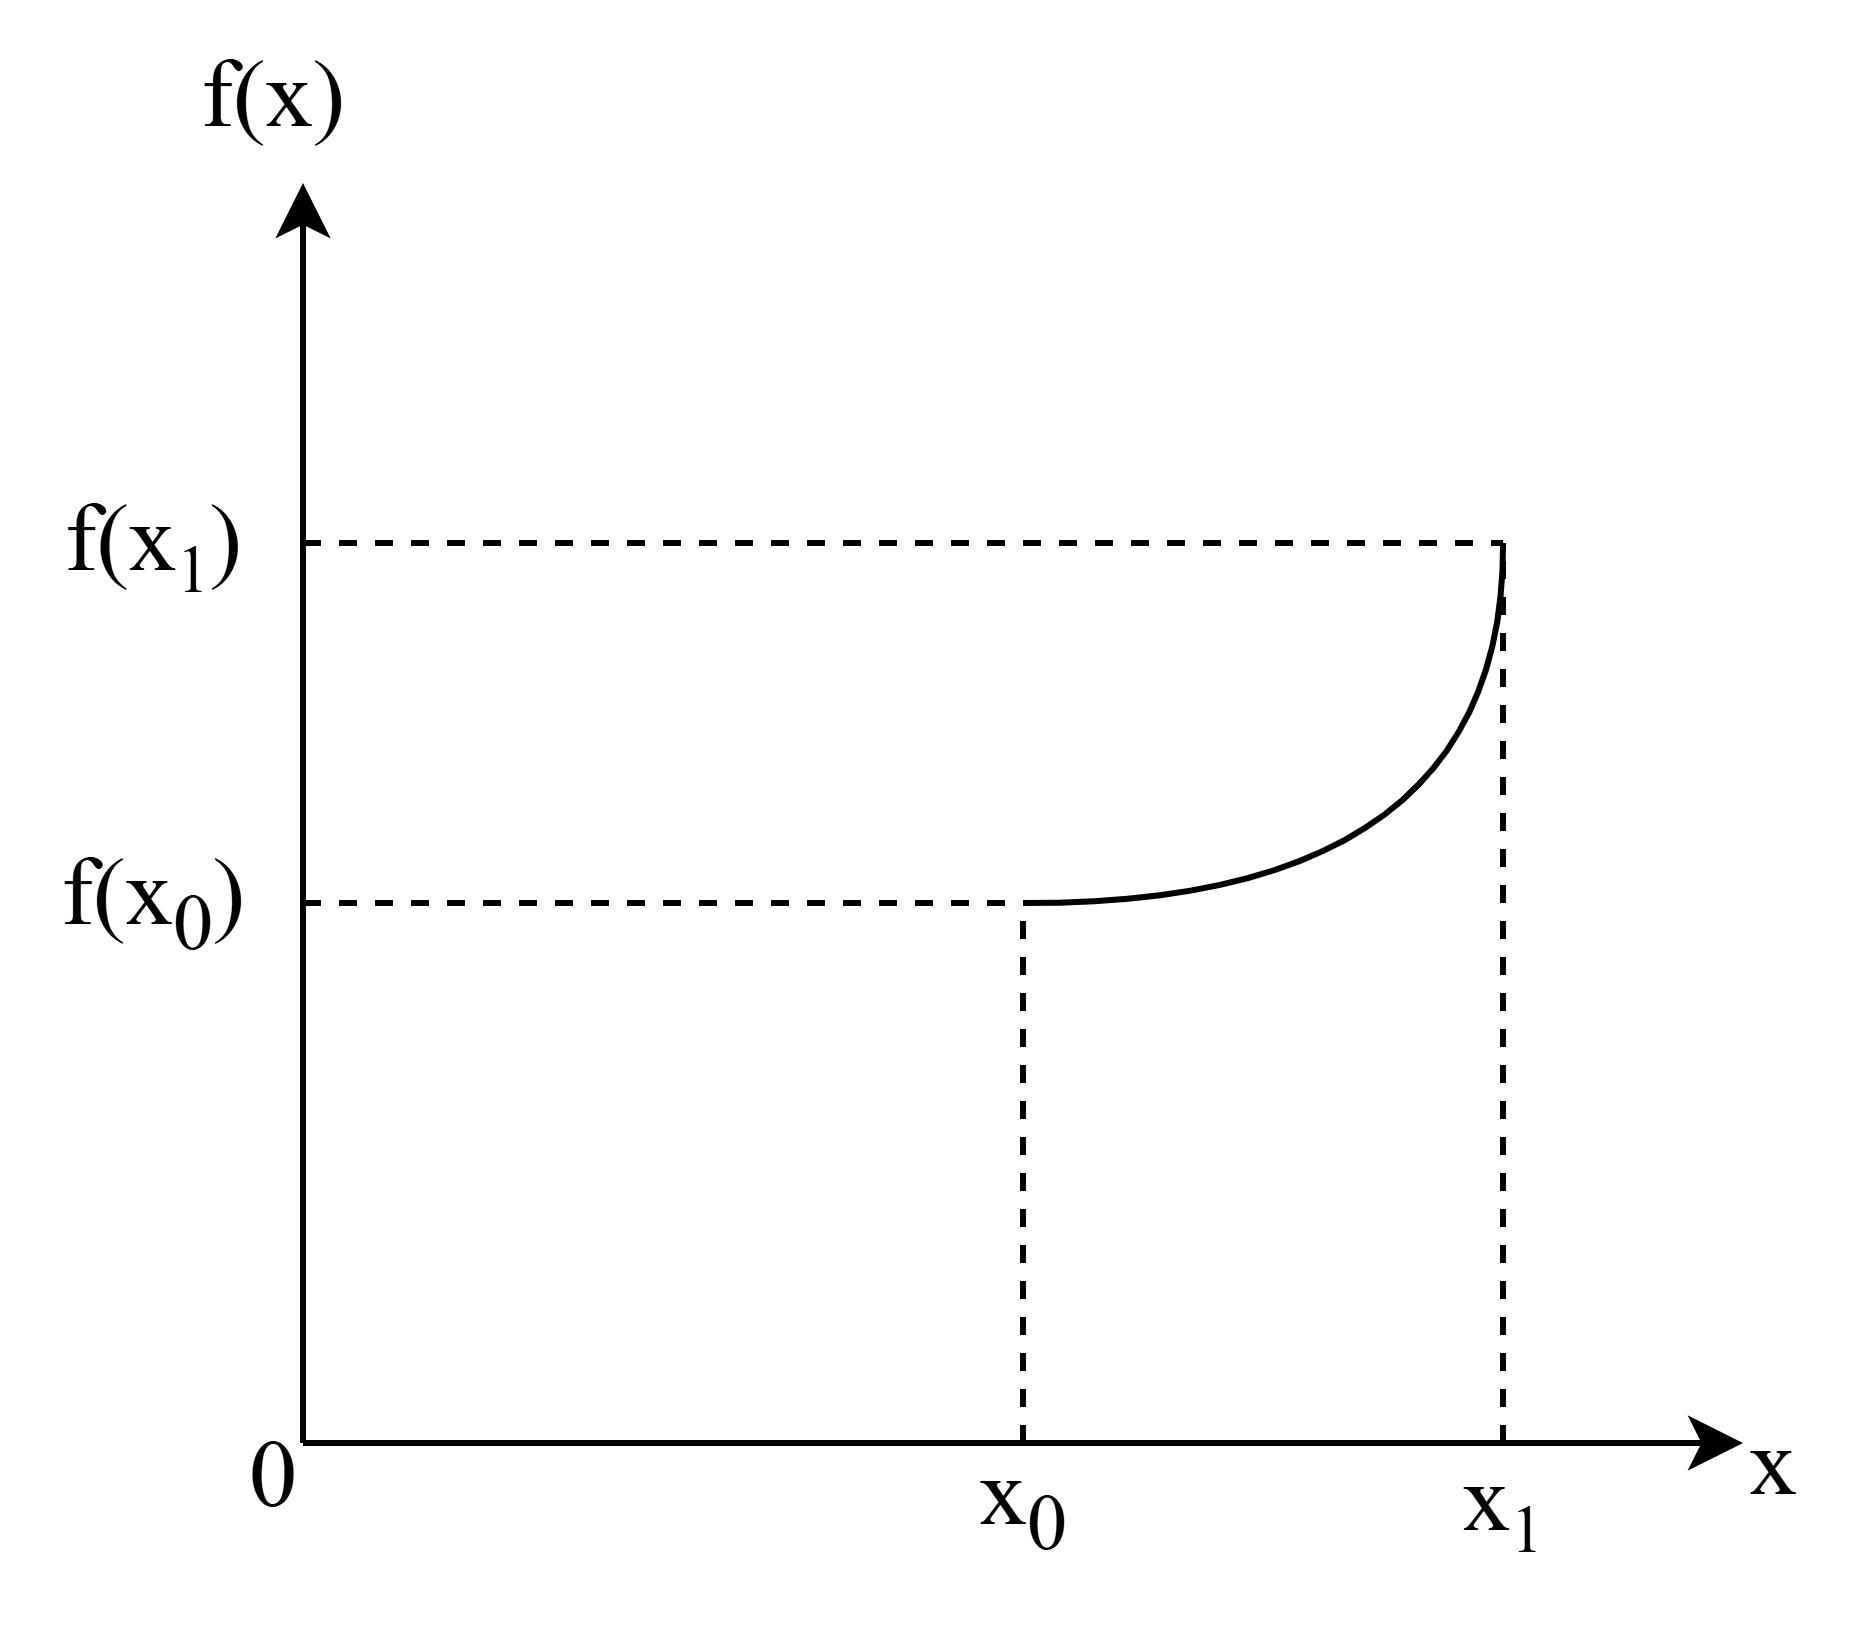
\includegraphics[width=0.4\textwidth]{images/3-1-1.png}
    \caption{Calculus of Variations: Varying a Curve}
    \label{fig:3-1-1}
\end{figure}

To extremize the functional $I[y(x)]$, we proceed as follows:

\begin{itemize}
    \item Fix the values of $y(x_0)$ and $y(x_1)$.
    \item Consider a curve $y(x)$ connecting these endpoints.
    \item Introduce a small perturbation to this curve:
    \[
        y(x) \rightarrow y(x) + \delta y(x)
    \]
    \item Compute the variation $\delta I$ under this perturbation, and require that the
    term linear in $\delta y$ vanishes.
    \item Since we have fixed the end points, we require $\delta y(x_0) = \delta y(x_1) = 0$.
\end{itemize}

Starting with the definition of the functional:

\[
    I[y(x)] = \int_{x_0}^{x_1} F(y(x), y'(x), x) \, dx
\]

The difference between the functional evaluated on the perturbed path and the original 
path is:

\[
    \delta I = I[y(x) + \delta y(x)] - I[y(x)] = \int_{x_0}^{x_1} \left( F(y + \delta y, y' + \delta y', x) - F(y, y', x) \right) dx
\]

Note that:

\begin{align*}
    y &\rightarrow y + \delta y \\
    y' &\rightarrow y' + \delta y' \\
\end{align*}

and thus:

\[
    \delta y' = (\delta y)'
\]

Using the first-order Taylor expansion of the function $F$ and the above equation, we get:

\begin{align*}
    \delta I &= \int_{x_0}^{x_1} dx \left( \frac{\partial F}{\partial y} \delta y + \frac{\partial F}{\partial y'} \delta y' \right) \\
    &= \int_{x_0}^{x_1} dx \left( \frac{\partial F}{\partial y} \delta y + \frac{\partial F}{\partial y'} \frac{d}{dx}(\delta y) \right)
\end{align*}

We can integrate the second term by parts, using the fact that 
$\int u \, dv = uv - \int v \, du$, where we set $u = \frac{\partial F}{\partial y'}$ 
and $dv = \frac{d}{dx}(\delta y)\, dx$:

\begin{align*}
    \delta I &= \int_{x_0}^{x_1} dx \left( \frac{\partial F}{\partial y} \delta y - \frac{d}{dx} \left(\frac{\partial F}{\partial y'}\right) \delta y \right) + \frac{\partial F}{\partial y'} \delta y \bigg|_{x_0}^{x_1}
\end{align*}

Since $\delta y(x_0) = \delta y(x_1) = 0$, the boundary term vanishes, and we have:

\begin{equation}
    \delta I = \int_{x_0}^{x_1} dx \left( \frac{\partial F}{\partial y} - \frac{d}{dx} \left(\frac{\partial F}{\partial y'}\right) \right) \delta y
\end{equation}

For $\delta I$ to be zero for an arbitrary perturbation $\delta y(x)$, the term inside
the parenthesis must vanish:

\begin{equation}
    \frac{\partial F}{\partial y} - \frac{d}{dx} \left(\frac{\partial F}{\partial y'}\right) = 0
\end{equation}

This is the \textbf{Euler-Lagrange Equation}. The quantity:

\begin{equation}
    \frac{\delta I}{\delta y(x)} = \frac{\partial F}{\partial y} - \frac{d}{dx} \left(\frac{\partial F}{\partial y'}\right)
\end{equation}

is called the functional derivative of $I[y(x)]$ with respect to $y(x)$.

Now, let's consider the generalization to a functional that depends on $N$ functions, 
rather than just one:

\begin{equation}
    I[y_i(x)] = \int dx F(y_i, \frac{dy_i}{dx}, x), \quad i = 1, 2, \dots, N
\end{equation}

The variation of this functional is given by:

\begin{equation}
    \delta I = \int dx \sum_{i=1}^{N} \left( \frac{\partial F}{\partial y_i} \delta y_i + \frac{\partial F}{\partial y'_i} \delta y'_i \right)
\end{equation}

Following the same procedure as before, we obtain:

\begin{equation}
    \delta I = \int dx \sum_{i=1}^{N} \left( \frac{\partial F}{\partial y_i} - \frac{d}{dx} \left(\frac{\partial F}{\partial y'_i}\right) \right) \delta y_i
\end{equation}

To minimize $I$ with respect to all $y_i(x)$, each $y_i(x)$ must satisfy the 
corresponding Euler-Lagrange equation:

\begin{equation}
    \frac{\delta I}{\delta y_i} = \frac{\partial F}{\partial y_i} - \frac{d}{dx} \left(\frac{\partial F}{\partial y'_i}\right) = 0
\end{equation}

for all $i$.

In conclusion, for a mechanical system with Lagrangian $L\left(q_i, \dot{q_i}, t\right)$,
the condition for the action $S[q_i(t)] = \int L\ dt$ to be extremized is

\begin{equation}
    \frac{\delta S}{\delta q_i} = \frac{\partial L}{\partial q_i} - \frac{d}{dt} \left(\frac{\partial L}{\partial \dot{q}_i}\right) = 0
\end{equation}

\begin{example}
    Prove that the shortest distance between two points is a line.
\end{example}

\begin{proof}
    The length of the path can be written as:
    \begin{equation}
        L = \int ds \sqrt{\left(\dot{x}^2 + \dot{y}^2\right)}
    \end{equation}
    Here $\dot{x}$ represents $\frac{dx}{ds}$.
    \begin{align}
        \frac{\delta L}{\delta x\left(s\right)} &= -\frac{d}{ds} 
        \left(\frac{\dot{x}}{\sqrt{\dot{x}^2 + \dot{y}^2}}\right) \\
        &= -\left(\frac{\ddot{x}}{\sqrt{\dot{x}^2 + \dot{y}^2}} - \frac{1}{2} 
        \frac{2\dot{x}^2\ddot{x}}{\left(\dot{x}^2+\dot{y}^2\right)^{\frac{3}{2}}}\right) \\
        &= 0
    \end{align}
    So we can get:
    \begin{equation}
        \ddot{x} \left(\dot{x}^2 + \dot{y}^2\right) - \dot{x}\left(\dot{x}\ddot{x} + \dot{y}\ddot{y}\right) = 0
    \end{equation}
    Which is:
    \begin{equation}
        \ddot{x} \dot{y}^2 - \dot{x} \dot{y} \ddot{y} = 0
    \end{equation}
    Similarly, if we take the derivative with respect to $y$, we get:
    \begin{equation}
        \ddot{y} \dot{x}^2 - \dot{x} \dot{y} \ddot{x} = 0
    \end{equation}
    From equation (3.14) we can get:

\end{proof}
